\begin{surferPage}[Septique de Labs]{Une Septique à 99 Singularités}
    En travaillant sur sa thèse à l'Université de Mayence en 2004, Oliver Labs 
    construisit une surface de degré $7$ (septique) à 99 singularités. Il s'agit du record actuel,
    mais il pourrait bien exister une septique ayant jusqu'à 104 singularités !
    La surface de Labs a comme symétries celles d'un heptagone régulier (image de gauche).
    Cela est bien visible en regardant la surface du dessus (image de droite) :

    \vspace*{-0.3em}
    \begin{center}
      \begin{tabular}{c@{\qquad}c}
        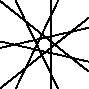
\includegraphics[height=1.5cm]{labsseptic1.pdf}
        &
        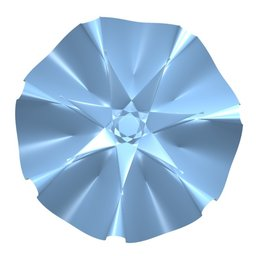
\includegraphics[height=1.5cm]{labs_septic_von_oben}
      \end{tabular}
    \end{center}
    \vspace*{-0.3em}

    Pour construire cette surface, Oliver Labs a utilisé le logiciel de calcul formel
    {\sc Singular} (Université de Kaiserslautern) particulièrement adapté pour les calculs
    en géométrie algébrique et en théorie des singularités.

    Il utilisa le fait qu'on peut effectuer des calculs de manière naturelle sur un ensemble 
    fini de nombres. Ceci est bien connu pour les horloges :
    24h $=$ 0h, 24h $+$ 1 heure n'est pas 25h, mais 1h.
\end{surferPage}
